\section{Verwandte Arbeiten}
\subsection{Verbesserungen des Ear-Clipping-Algorithmus}

Wenn man einen Algorithmus mathematisch betrachtet, dann ist die Zeit, welcher er bis zur Terminierung benötigt, zumeist der
Gegenstand der Betrachtung. Mittels der Komplexitätstheorie lässt sich diese, vom Typ des Computers, auf welchem der Algorithmus 
läuft, unabhängig, beschreiben. Das Referenzmodell ist dabei zumeist die \ac{tm}.\cite{tm} Ziel ist es, dass ein Algorithmus 
auf einer \ac{tm} in Polynomialzeit abläuft. Diese Zeit hängt zumeist von der Eingabegröße ab. Für den \ac{eca} ist die entscheidende 
Größe die Anzahl der Ecken $n$ des Polygons $P$.
Betrachtet man den \ac{eca} auf einer \ac{tm}, so hat er eine Komplexität von $O(n^3)$.
Zwar ist dieser Term ein Polynom in $n$, jedoch ist das kein Grund für die Wissenschaft, hier mit der Optimierung aufzuhören.
Wie O'Rourke in seiner Arbeit zeigt, kann man den \ac{eca} durch kleine Änderungen so modifizieren, dass dieser eine Komplexität von $O(n^2)$
aufweist.\cite{orourke} Diese Erkenntnis nutzen Mei, Tipper und Xu, um den Algorithmus auf andere Art zu verbessern.\cite{earclipping}

Für einen Algorithmus wie den \ac{eca} ist nicht nur seine Laufzeit entscheidend. Während andere Algorithmen beispielsweise Entscheidungsprobleme lösen, 
bei denen es nur um die Frage nahc der Existenz der Lösung geht, ist bei einer Triangulation bereits bekannt, dass es unterschiedliche Lösungen gibt.
Daher ist die Frage nicht, ob eine Lösung existiert, sondern ob eine optimale solche gefunden werden kann. Optimal ist dabei ein relativer Begriff, 
der stark von den Rahmenbedingungen abhängt. Für den \ac{eca} ist der Speicherbedarf ebenfalls entscheidend. Dieser ist bei Mei, Tipper und Xu durch $O(n)$
begenzt. Das Ziel ihrer Arbeit war es, qualitytiv hochwertige Triangulationen für komplexe Polygone zu erzeugen. Der Qualitätsparameter war dabei der kleinste 
Innenwinkel der erzeugten Dreiecke in der Zerlegung. Genauer ging es darum, die sogenannten Slivers zu vermeiden (s. Kapitel 2.3).

Ihr Ansatz war es, den verbesserten Algorithmus von O'Rourke so zu modifizieren, dass er über die Option des \textbf{Edge Swappings} verfügt.
Wird ein Ear erkannt, dann wird für jeden seiner Innenwinkel überprüft, ob dieser kleiner ist als ein zuvor festgelegter Grenzwert. Ist das der Fall, dann 
muss bei diesem Dreieck Edge Swapping durchgeführt werden. Dafür werden der größte Innenwinkel des Dreickes und die, ihm gegenüberliedende, längste Seite bestimmt.
Daraufhin wird überprüft, ob es ein Nachbardreieck gibt, welches sich mit dem Ursprünglichen eben diese längste Seite teilt. Gibt es einen solchen Nachbarn, 
dann wird in dem von den beiden Dreiecken gebildeten Viereck eine Diagonale zwischen den beiden Ecken gezogen, welche jeweils der zuvor bestimmten längsten Seite gegenüber lagen.
Auf diese Art entstehen wieder zwei Dreiecke, von denen nun die Innenwinkel auf ihre Größe überprüft werden. Ist jeweil der kleinste Winkel größer als der Grenzwert, 
dann ist die Qualität der Dreicke nun besser als die des ursprünglich Ausgewählten. Wenn dem nicht so ist, bleibt alles unverändert und das Ear wird wie es war gewählt und abgeschnitten.

\begin{figure}[h]
    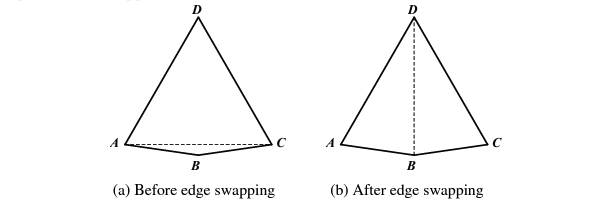
\includegraphics[width=1\textwidth]{bilder/edgeswapping.png}
    \caption[Edge Swapping]{Edge Swapping \cite{earclipping}}
    \label{fig:edgeswapping}
\end{figure}

Auf diese Art kann die Qualität der Dreiecke in der Triangulation stark erhöht werden. Sie zeigen an Beispielen, dass sich die Innenwinkelgröße durchschniitlich verdoppelt.
Teilweise können Dreiecke mit minimalem Innenwinkel von $< 15^\circ$ ganz eliminiert werden. Das hängt jedoch vom eingegebenen Poylgon ab und hat keine Allgemeingültigkeit.

\subsection{Parallelisierung des Ear-Clipping-Algorithmus}

Anstatt den Algorithmus selbst in seiner Laufzeit zu verbessern, ist es ein Gedanke, die Abarbeitung aufzuteilen. Vorallem mit der technischen Entwicklung mehrerer Prozessorkerne in einer \ac{cpu},
ist verteiltes Rechnen ein gängiges Konzept. Hierzu haben Eder, Held und Palfrader eine Arbeit verfasst, die sich mit der Umsetzung des \ac{eca} unter dem Gesichtspunkt der coarse-grain parallelization,
zu Deutsch grobkörnigen Parallelisierung, befasst.\cite{paralleleca} Dieses Prinzip beschreibt die Aufteilung eines Programms in längere Unteraufgaben. Das ist ein für Multicore Computer sehr geeignetes Konzept.
Andere Arbeiten befassten sich auch mit der Umsetzung der Arbeitsteilung aber dort speziell mit dem Konzept der fine-grain parallelization im Bezug auf die \ac{dt}. Die fine-grain parallelization, also die feinkörnige 
Parallelisierung, beschreibt die Aufteilung eines Programms in eine Vielzahl kleinerer Aufgaben. 
Hier ist beispielsweise M. Goodrich\cite{goodrich} zu nennen.

Eder, Held und Palfrader haben ihre Arbeit auf \ac{fist} aufgebaut. Dieses Framework ist ein in C++ verfasster Code für Polygontriangulation basierend auf dem \ac{eca}.\cite{paralleleca}
Sie beschränkten sich dabei mit der Parallelisierung auf den Bereich des Algorithmus, welcher sich mit der Klassifikation und dem Clipping der Ears befasst. Dieser Teil mach etwa $80\%$ des Rechenaufwandes aus.
Um eine Aufteilung in $k$ Threads zu erreichen, welche dann auf den $k$ Kernen der \ac{cpu} abgearbeitet werden sollen, nutzen Sie drei verschiedene Ansätze und vergleichen diese miteinander und mit der nicht parallel 
laufenden Form des Algorithmus in \ac{fist}.

Ihr erster Ansatz beruht auf dem \emph{devide-and-conquer-Prinzip}. Anstatt das Polygon $P$ allerding durch Diagonalen in etwa gleich große Unterpolygone $P_k$ zu unterteilen, 
nutzen Sie $k-1$ viele senkrechte Geraden dafür. Dies ist weit weniger aufwendig in der Berechnung, da das Finden von geeigneten Diagonalen relativ rechenintensiv ist.
Sie berufen sich dabei auf einen Algorithmus von Sutherland und Hodgman \cite{dnc}. Bei dieser Form der Unterteilung enstehen sogenannte \ac{sp}, welche die Schnittpunkte der senkrechten Geraden mit 
den Strecken der äußeren Begrenzung darstellen. Dafür benötigt man eine Zeit von $O(n)$ pro Gerade $l$ und fügt im schlimmsten Fall $O(n)$ \ac{sp} ein. Diese werden als neue Eckpunkte in den Unterpolygonen eingefügt und damit vom \ac{eca} auch als Eckpunkte der Dreicke in der Zerlegung benutzt. 
Das führt dazu, das Dreiecke in der Gesamtzerlegung von $P$ entstehen, welche unzulässige Eckpunkte besitzen, da diese im Ursprünglichen Polygon nicht existieren. 
Dafür muss eine Bereinigung der Zerlegung durchgeführt werden, nachdem alle $k$ Threads ihre Triangulation der $P_k$ Unterpolygone geliefert haben. 
Durch den Schnitt des Poylgons mit einer senkrechten Geraden entstehen zwei \ac{sp} $s_a$ und $s_b$. Um diese wieder zu löschen, werden alle Dreiecke, welche zu einem dieser beiden Punkte inzident sind, aus der Triangulation 
gelöscht. Auf diese Weise erzeugt man ein Loch $H$ in der Zerlegung, welches wieder ein Polygon ist. Diese kann man nun durch erneute Triangulation mit validen Dreiecken füllen. \linebreak 

Einen \emph{partition-and-cut-Ansatz} zu verwenden, war die zweite Variante, um die Triangulation auf die $k$ Threads aufzuteilen. Dabei wird nicht wie bei \emph{divide-and-conquer} das gesamte Polygon $P$, sondern nur sein begrenzender Streckenzug unterteilt.
Hierfür werden \textbf{Landmarks}, also Wegpunkte, eingeführt. Dies geschieht anhand der Indizierung der $n$ Ecken. Die Eckpunkte mit den Indizes $\left\{ 0, \frac{n}{k}, \frac{2n}{k}, \dots, \frac{(k-1)n}{k} \right\}$ werden die Landmarks. Der Streckenzug zwischen je zwei dieser Markierungen wird 
jeweils einem Thread zugewiesen. Die Wegpunkte gehören dabei jeweils zu zwei benachtbarten Teilstreckenzügen gleichzeitig. Jeder Thread durchläuft dann eine Klassifikations- und eine Clippingphase, bei denen darauf geachtet wird, dass die Landmarks nicht gelöscht werden.
Ist das geschehen und alle Threads beendet, dann bleibt ein Teil des Polygons noch unbearbeitet. Dieser Teil wird bei Eder, Held und Palfrader nicht nocheinaml in Abschnitte für verschiedene Threads unterteilt sondern wird dann vom sequentiellen \ac{eca} in \ac{fist} bearbeitet.
Zwischen den Threads wird keine Synchronisation benötigt, da sowohl Klassifikation als auch Clipping völlig undabhängig von anderen Threads ablaufen und nur in ihrem jeweiligen Abschnitt Dreiecke erzeugt werden. Dabei sei angemerkt, dass das Überprpüfen der Ear-Eigenschaft nur Lesezugriff auf 
die Globale Liste aller Eckpunkte des Polygons benötigt. Der Vorgang der Aufteilung in Threads und deren bearbeitung ist in der nachstehenden Abbildung zu sehen. \linebreak
\begin{figure}[h]
    \centering
    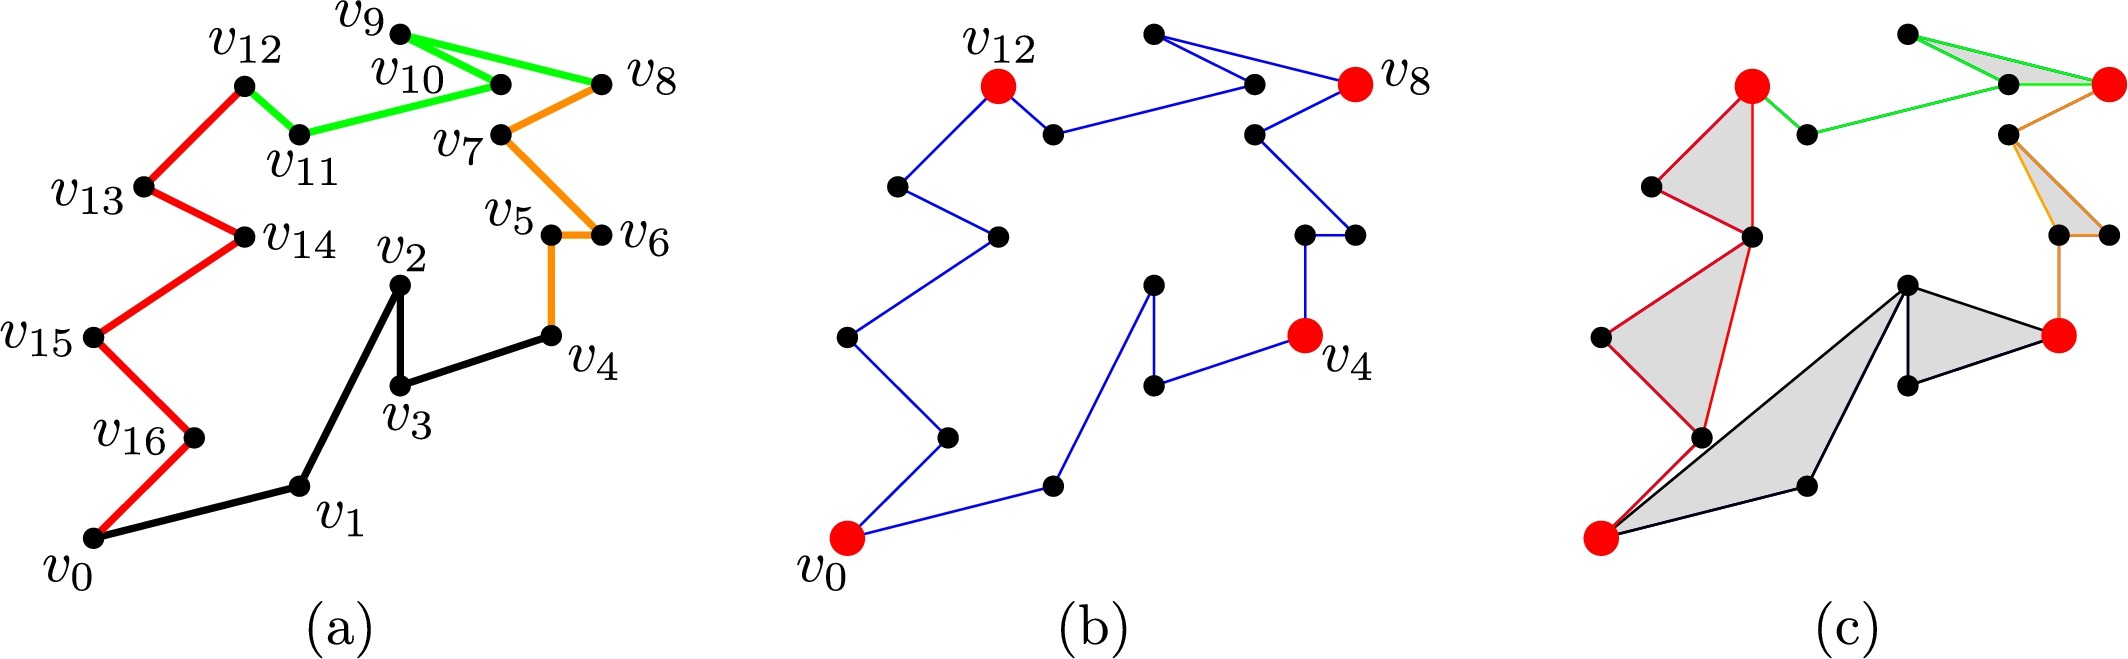
\includegraphics[width=0.8\textwidth]{bilder/segmentierung.jpg}
    \caption[Unterteilung des Streckenzugs in Unterstreckenzüge mittels Landmarks für Parallelisierung]{\centering (a) Einfaches Polygon $P$ unterteilt in vier Streckenzüge (b) Landmarks vervorgehoben (c) Triangulierung durch Threads}
    \label{fig:langmarks}
\end{figure}

Der dritte Ansatz, betreffend dem \ac{eca} in \ac{fist} ist der sogenannte \emph{mark-and-cut-Ansatz}, welcher Ähnlichkeiten zum vorher erwähnten \emph{partition-and-cut-Ansatz} aufweist. Auch in diesem Fall werden einige Eckpunkte von $P$ als Markierungen genutzt.
In der Marierungsphase, durchläuft ein Thread den Streckenzug von $P$ und speichert jeden zweiten konvexen Eckpunkt in einer Liste. Hat dieser Thread die Hälfte aller Punkte überprüft, werden die Cut-Threads gestartet, welche nur die Cutting-Phase durchlaufen. Bildet 
ein Punkt in der Liste mit seiner gegenüberliegenden Seite ein Dreicke, dann wird dieses sofort als valide gespeichert und abgeschnitten. Jeder dieser Punkte darf nur einmal bearbeitet werden, damit es nicht zu Asynchronität und Redundanz kommt. Wenn die Cut-Threads alle ihre Arbeit getan haben, 
werden sie neu gestartet und bearbeiten dann alle Punkte, die Seit ihrem letzten Start zur Liste hinzugefügt worden sind.
Während dessen durchläuft der Mark-Thread das Polygon erneut und fürgt neue konvexe Punkte zu Liste hinzu und so weiter, bis nurnoch weniger Dreiecke erkannt werden, als vorher mit einem Grenzwert festgelegt. Dieser lag bei Eder, Held und Palfrader bei 20 Dreiecken.
Der Rest von $P$, welcher noch nicht bearbeitet wurde, wird dann wie im \emph{partition-and-cut-Ansatz} von einem sequentiellen Aufruf von \ac{fist} bearbeitet. 

\begin{figure}[b]
    \centering
    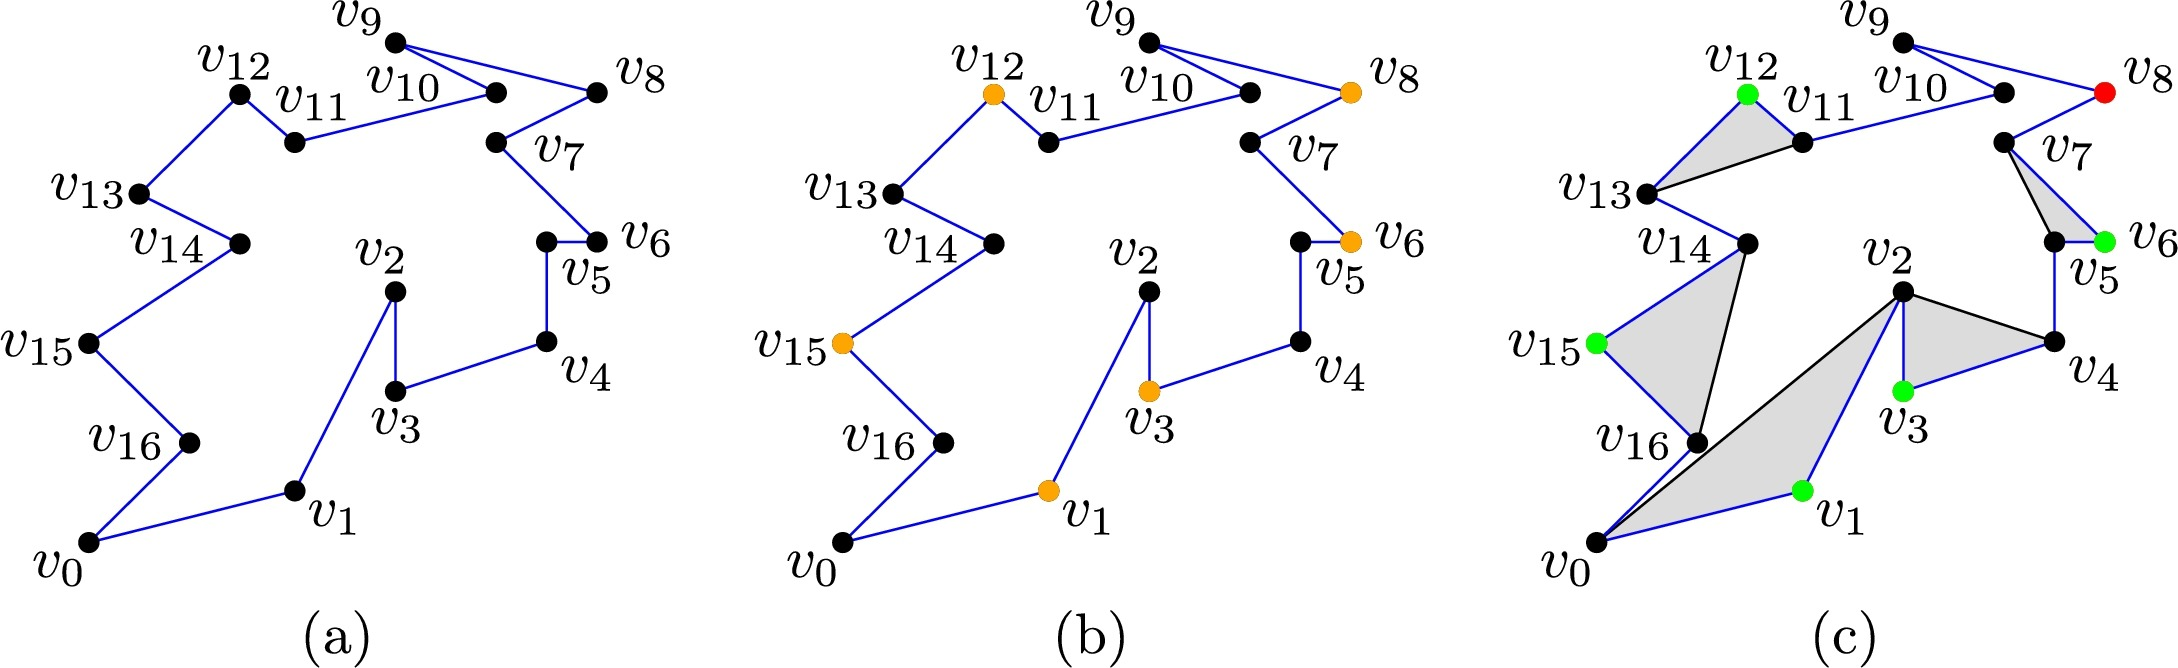
\includegraphics[width=0.8\textwidth]{bilder/markierung.jpg}
    \caption[Markierung konvexer Eckpunkte für Parallelisierung]{\centering (a) Einfaches Polygon $P$ (b) Erste Markierungsphase, ausgewählte Ecken in orange (c) Erste Cutting-Phase}
    \label{fig:konvPoints}
\end{figure}

Der finale Vergleich aller drei Ansätze hinsichtlich ihrer Qualität zeigt, dass sie in etwa gleich gut sind. Als Vergleich wurde von ihnen noch eine Variante der \ac{dt}, die sogenannte \ac{cdt} durchgeführt, auf die an dieser Stelle allerdings nicht 
genauer eingegangen werden soll. Die folgende Tabelle zeigt das Ergebnis.

\begin{table}[h]
    \begin{tabular}[h]{| l | c | c | c | c | c |}
    \hline
    & CDT & FIST's top & D\&C & P$\&$C & M$\&$C \\ \hline
    (1) Durchschn. Abw. 60° & 30.79° & 31.53° & 35.29° & 34.97° & 38.38° \\ \hline
    (2) Durchschn. min. Winkel & 24.60° & 23.40° & 20.07° & 21.32° & 21.07° \\ \hline
    \end{tabular}
    \caption[Vergleich verschiedener Parallelisierungen des \ac{eca} in \ac{fist}]{Vergleich der \ac{fist} Trianulation inklusive \ac{cdt} und FIST's top Heuristik. Aufgeführt sind folgende Parallele Versionen von \ac{fist}: 
    Divide-and-conquer D\&C, Partition-and-cut P\&C und Mark-and-Cut M\&C. 
    (1) Durchschnittliche Abweichung aller Innenwinkel von 60° über alle Triangulationen (je kleiner, desdo besser) 
    (2) Durchschnittliche Größe des kleinsten Innenwinkels aller Dreicke über alle Trinagulationen (je größer, desdo besser) \cite{paralleleca}}
    \label{tab:tab1}
\end{table}

\subsection{Alternative Verfahren und Ansätze} 

\subsubsection{Delauny Triangulation}



\subsubsection{Algorithmus basierend auf Sichtbarkeit}

Wie schon bei der \ac{dt} ist hier der Begriff der Sichtbarkeit von Eckpunkten entscheidend. Anders als zuvor werden hier jedoch nicht sofort Dreicke ermittelt,
welche die Bedingung des leeren Umkreises erfüllen. In diesem Algorithmus, beschrieben von Ran Liu, wird das Polygon $P$ in zwei Unterpolygone $P_1$ und $P_2$ unterteilt,
welche dann solange rekursiv weiter unterteilt werden, bis die entstandenen Unterpolygone $P_i$ Dreiecke sind.\cite{newAlg}
Hierfür muss in einem ersten Schritt die Sichtbarkeit jedes Punkte gegenüber einem Referenzpunkt $v_i$ überprüft werden. Dazu betrachtet man zunächst die Nachbarn $v_{i-1}$ und $v_i+1$ 
von $v_i$. Diese begrenzen das sogenannte \textbf{Sichtfeld} von $v_i$, welches mit $\alpha$ bezeichnet wird und dem Winkel in $v_i$ entspricht. Für spätere Betrachtungen zählen $v_{i-1}$ und $v_{i+1}$ 
als nicht sichtbar im BEzug auf $v_i$. Entlang der Kanten von $P$ wird nun ausgehend von $v_{i+1}$ entgegen dem Uhrzeigersinn überprüft, ob ein Punkt $v_j$ im Sichtfeld von $v_i$ liegt.
Ist das der Fall, dann gilt der Punkt $v_j$ als sichtbar, wenn die Strecke $v_iv_j$ eine Diagonale von $P$ ist. Zusätzlich begrenzt dieser Punkt nun das Sichtfeld und es muss verkleinert werden. Das neue Sichtfeld $\alpha$ berchnet sich also durch $\alpha = v_{i-1},v_i,v_j$.
Der Vorgang wird fortgesetzt, bis alle Punkte überprüft sind. Ist diese Überprüfung für alle $v_i$ von $P$ abgeschlossen, wird die Anzahl der sichtaberen Punkte 
gegenüber dem jeweiligen Referenzpunkt bestimmt. Diese dient als Vergleichskriterum für die Punkte untereinander. Als Beispiel ist in der nachfolgenden Abbildung einmal die Ermittlung von $alpha$ und die Überprüfung 
mehrerer Punkte bezogen auf den Punkt $v_0$ dargestellt.

\begin{figure}[t]
\centering
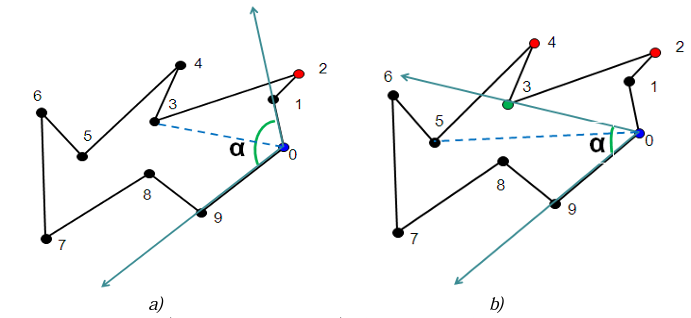
\includegraphics[width=1\textwidth]{bilder/sichtbarkeit.png}
\caption[Sichtbarkeit von Punkten]{\centering(a) $v_3$ ist sichtbar für $v_0$ (b) Überprüfung der Sichtbarkeit von $v_5$ mit neuem Sichtfeld $\alpha$ (nicht sichtbar entspricht rot, sichtbar entspricht grün) \cite{newAlg} }
\label{fig:visibPoint}
\end{figure}

Für die Anzahl sichtbarer Punkte bezogen auf $v_i$ wird die hier Bezeichnung $s(v_i)$ verwendet. Man kann diesen Vorgang der Sichtbarkeitsanalyse wie folgt in Pseudocode beschreiben.

\begin{flushleft}
    { \textbf{Algorithmus 3: Sichtbarkeitsanalyse für einen Punkt $v_i$}
          \begin{tabbing}
            \=$~~~~~~$ \= \textbf{Eingabe:} $~~~$\=  Eck\=en $v_i$\=$ \in V$\=$(P),~n = |V(P)| - 3,~s(v_i)=0$\\
            \> \> \textbf{Ausgabe:} \> Anzahl sichtbarer Punkte $s(v_i)$\\
            \> \> \textbf{Schritt 1:} \> Wähle Referenzpunkt $v_i$ \\
            \> \> \textbf{Schritt 2:} \>$\alpha = \angle v_{i-1}v_iv_{i+1}$\\
            \> \> \textbf{Schritt 3:} \>\textbf{while} $n > 0$ \textbf{do}\\
            \> \> \> \> \textbf{if} $\angle v_{i-1}v_iv_j > 0 \wedge \angle v_{i-1}v_iv_j < \alpha$\\
            \> \> \> \> \> \textbf{if} $v_iv_j$ Diagonale von $P$\\
            \> \> \> \> \> \> (a) $s(v_i)= s(v_i)+1$\\
            \> \> \> \> \> \> (b) $\alpha = \angle v_{i-1}v_iv_j$\\
            \> \> \> \> \> \> (c) $n = n-1$\\
            \> \> \textbf{Schritt 4:} \> Ausgabe von $s(v_i)$ 

          \end{tabbing}
  }
  \end{flushleft}

Ist $s(v_i)$ für jeden Eckpunkt $v_i$ von $P$ ermittelt, wird der Punkt mit der größten solchen Anzhal ausgewählt. Gibt es mehrere solche Punkte, dann 
kann ein beliebige dieser Punkte gewählt werden. Dieser Punkt wird dann als \textbf{First Head} bezeichnet.
Als nächstes wird noch der Punkt mit der zweit höchsten Anzahl $s(v_i)$ gewählt. Er wird als \textbf{Second Head} bezeichnet. Sollte es hier Uneindeutigkeiten
bei der Auswahl geben, dann wird ein Test durchgeführt, um diesen Punkt auszuwählen. Durch die Diagonale zwischen First und Second Head soll das Polygon in zwei 
Unterpolygone zerlegt werden. Man testet, bei welchem der möglichen Punkte für den Second Head, der Betrag der Differenz zwischen der Anzahl an Strecken in den beiden 
Unterpolygonen $P_1$ und $P_2$ am geringsten ist. Das ist in der nächsten Abbildung zu sehen.

\begin{figure}[t]
    \centering
    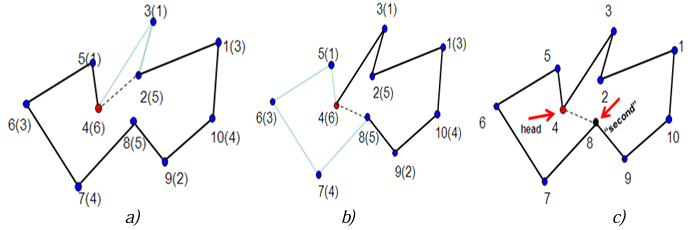
\includegraphics[width=1\textwidth]{bilder/second_head_comp.png}
    \caption[Test zur Auswahl des Second Head]{\centering(a) und (b) Vergleich der Differenz zwischen der Länge des schwazen und des türkiesen Strecknabschnitts (c) Auswahl des Second Head \cite{newAlg} }
    \label{fig:secHead}
\end{figure}

Für die Zerlegung werden First und Second Head dann dupliziert, damit beide Polygone vollständig begrenzt sind. In beiden Unterpolygonen muss dann die Sichtbarkeitsanalyse erneut durchgeführt werden.
Damit dies ein wenig schneller geschieht, kann man die sichtbaren Punkte im Bezug auf einen Punkt $v_i$ in einer sogennanten \emph{single circular list} gespeichert werden. In einer solchen Liste zeigt der Pointer des 
letzten Elements auf das erste Element der Liste. Beim Update der Sichtbarkeiten müssen dann für jeden Punkt nur die Punkte in seiner jeweiligen Liste überprüft werden und jetzt nicht mehr sichtbare Punkte aus der Liste 
gelöscht werden. Damit wird die Laufzeit der Sichtbarkeitsanalyse von $O(n^2)$ auf $O(n)$ begrenzt. Nichtsdesdotrotz hat der neue Algorithmus von Ran Liu, nach seiner eigenen groben Analyse, eine Komplexität von über $O(n^3)$.
Im Vergleich mit dem \ac{eca}, welcher eine Komplexität von $O(n^2)$ besitzt, schneidet er damit schlechter ab. In Tabelle \ref{tab:tab2} und \ref{tab:tab3} werden zwei Beispiele des Vergleichs zwischen dem Sichtbarkeitsalgorithmus 
und dem \ac{eca} aus der Arbeit von Liu angeführt. Die Algorithmen wurden auf zufällig generierten Polygone unterschiedlicher Knotenanzahl und Form getestet. Dabei waren die getesteten Polygonformen einmal \emph{rund}, das heißt 
die Eckpunkte konnten nur in einem quadratischen Koordinatenbereich liegen. Der andere Typ war \emph{länglich}, wobei die Punkte eher in ihrer x-Koordinate weiter streuten, nicht so sehr jedoch in der y-Koordinate.
Es ist in den Ergebnissen dieser Tests ersichtlich, dass die Qualität der Dreicke bezogen auf ihre minimalen Innenwinkel bei Liu's Algorithmus besser ist, als die des \ac{eca}. In Sachen Laufzeit jedoch schneitet der neue Algorithmus jedoch schlechter ab,
wie bereits die Komplexitätsanalyse zeigte.

In der nachfolgenden Abbildung ist zunächst einmal exemplarisch dargestellt, wie eine solche Zerlegung eines einfachen Polygons durchgeführt wird.
Danach folgen die angesprochenen Tabellen.
\begin{figure}[t]
    \centering
    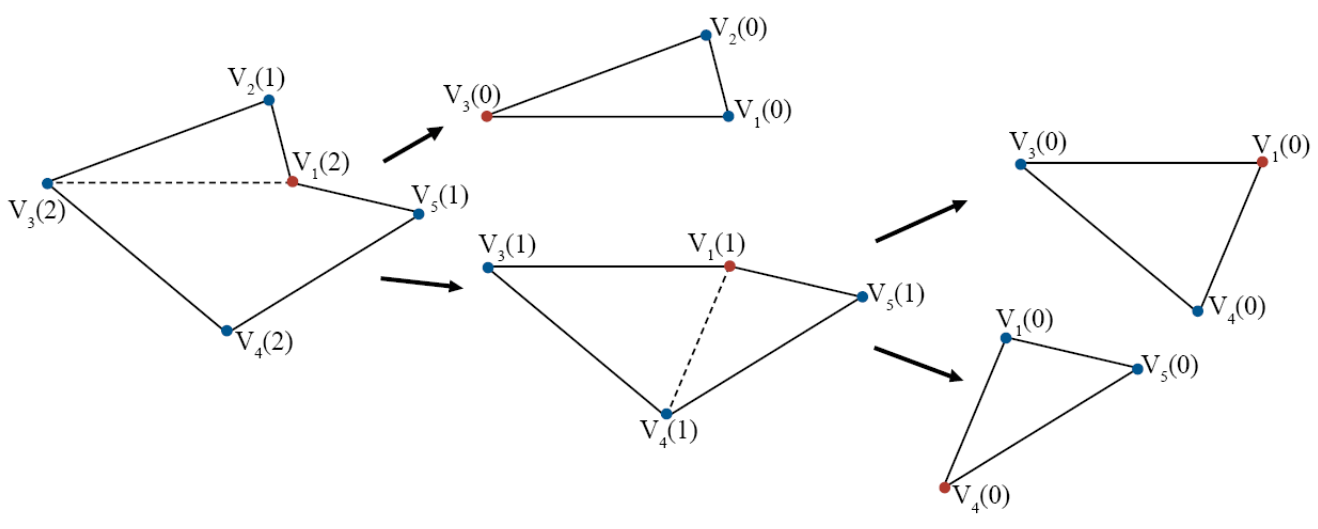
\includegraphics[width=1\textwidth]{bilder/sichtbarkeit_zerlegung.png}
    \caption[Triangulation mittels Sichtbarkeitsalgorithmus]{\centering Von links nach rechts die Schritte der Unterteilung eines Polygons in Unterpolygone bis zur Triangulierung mittels Sichtbarkeit der Eckpunkte (rot die First Heads)\cite{newAlg} }
\end{figure}

\begin{table}[ht]
    \begin{tabular}[ht]{| c | c | c | c | c |}
    \hline
    \multicolumn{5}{|c|}{Eckenanzahl: 30 ~~~ $v_i = \left\{(x,y)| -50 < x < 50, -50 < y < 50\right\}$}\\ \hline
   Algorithmus & Polygon- & Durchschn.& Standartabw. & Durchschn. \\
   & fläche &  Dreiecksfläche & der Dreiecksfläche & min. Winkel \\ \hline
    Ear-Clipping & 4128,5px & 147,446px  & 163,63px  & 10,29° \\ \hline
    Sichtbarkeit & 4128,5px & 147,446px  & 148,91px & 15,04°\\ \hline
    \end{tabular}
    \caption[Vergleich \ac{eca} und Sichtbarkeitsalgorithmus bei rundem Polygon]{\centering Vergleich des \ac{eca} und des Sichtbarkeitsalgorithmus bei einem rundem Polygon mit 30 Ecken anhand der Standartabweichung der Dreiecksfläche in Pixeln (je kleiner desdo besser)
    und der durchschnittlichen minimalen Innenwinkelgröße in Grad (je größer desdo besser)\cite{newAlg}}
    \label{tab:tab2}
\end{table}

\begin{table}[b]
    \begin{tabular}[b]{| c | c | c | c | c |}
    \hline
    \multicolumn{5}{|c|}{Eckenanzahl: 30 ~~~ $v_i = \left\{(x,y)| -100 < x < 100, -30 < y < 30\right\}$}\\ \hline
   Algorithmus & Polygon- & Durchschn.& Standartabw. & Durchschn. \\
   & fläche &  Dreiecksfläche & der Dreiecksfläche & min. Winkel \\ \hline
    Ear-Clipping & 5066px & 180,93px & 185,50px & 9,23° \\ \hline
    Sichtbarkeit & 5066px & 180,93px & 146,03px & 16,45° \\ \hline
    \end{tabular}
    \caption[Vergleich \ac{eca} und Sichtbarkeitsalgorithmus bei länglichem Polygon]{\centering Vergleich des \ac{eca} und des Sichtbarkeitsalgorithmus bei einem länglichen Polygon mit 30 Ecken anhand der Standartabweichung der Dreiecksfläche in Pixeln (je kleiner desdo besser)
    und der durchschnittlichen minimalen Innenwinkelgröße in Grad (je größer desdo besser) \cite{newAlg}}
    \label{tab:tab3}
\end{table}

